% Work-MAT | 2. rocnik | pripravovana hodina 47
% Návaznost: uživatelské připravy.zip (hodiny 01–20), autorská učebnice na GitHubu.
% Realisticky.cz: didaktická inspirace v posloupnosti a typech úloh; zadání jsou vlastní.
\documentclass[11pt,a4paper]{article}
\input{../../sablony/pripravy/priprava.sty}
\usepackage{tikz}
\nastavPripravu{2. ročník}{Orientovaný úhel}{47}{Orientovaný úhel}
\begin{document}
\blok{Motivace a návaznost}
Základní úhel chápeme jako otočení polopřímky od kladného směru osy $x$ kolem počátku. Nech žáky proti sobě zakreslit kladnou a zápornou orientaci.
\poznamka{Orientační nabídka pro 45--55 minut: krátké zopakování a motivace, nový výklad, tři společné vzorové úlohy, samostatná práce. Vyber podle tempa třídy; zbývající zadání slouží jako rezerva.}
\blok{Výklad}
V kladném směru obíhá úhel proti hodinovým ručičkám. Úhly lišící se o celé otočky mají stejné koncové rameno.
\begin{center}
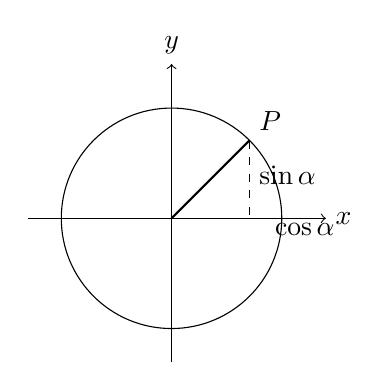
\begin{tikzpicture}[scale=1.4]
\draw[->] (-1.3,0)--(1.4,0) node[right] {$x$};
\draw[->] (0,-1.3)--(0,1.4) node[above] {$y$};
\draw (0,0) circle (1);
\draw[thick] (0,0)--(0.7071,0.7071);
\draw[dashed] (0.7071,0.7071)--(0.7071,0);
\node[above right] at (0.7071,0.7071) {$P$};
\node[below right] at (0.85,0.04) {$\cos\alpha$};
\node[right] at (0.7071,0.39) {$\sin\alpha$};
\end{tikzpicture}
\end{center}
\blok{Společné příklady}
\begin{prikladReseniBox}[title={Příklad 1}]
Vyřeš, resp. urči: $-45^\circ\text{ převedeme na úhel v }[0;360^\circ)$.
\tcblower
\[\begin{aligned}-45^\circ+360^\circ=315^\circ\end{aligned}\]
\end{prikladReseniBox}
\begin{prikladReseniBox}[title={Příklad 2}]
Vyřeš, resp. urči: $750^\circ\text{ převedeme na základní otočku}$.
\tcblower
\[\begin{aligned}750^\circ-2\cdot360^\circ=30^\circ\end{aligned}\]
\end{prikladReseniBox}
\poznamka{Nakresli na tabuli orientovanou kružnici a ukaž rozdíl mezi $+90^\circ$ a $-90^\circ$.}
\blok{Samostatné procvičování}
\begin{zadaniReseniBox}[title={Samostatná práce 1}]
\begin{enumerate}[label=\alph*)]
\item $-90^\circ\text{ na radiány}$.
\item $\frac{3\pi}{4}\text{ na stupně}$.
\item $225^\circ\text{ na radiány}$.
\item $-45^\circ\text{ jako kladný úhel}$.
\item $390^\circ\text{ po jedné otočce}$.
\item $-120^\circ\text{ jako kladný úhel}$.
\end{enumerate}
\tcblower
\begin{enumerate}[label=\alph*)]
\item $-\frac{\pi}{2}$.
\item $135°$.
\item $\frac{5\pi}{4}$.
\item $315°$.
\item $30°$.
\item $240°$.
\end{enumerate}
\end{zadaniReseniBox}
\blok{Dobrovolné rozšíření}
\begin{zadaniReseniBox}[title={Rozšíření 1}]
\begin{enumerate}[label=\alph*)]
\item Navrhni obdobnou úlohu s jiným úhlem a zkontroluj výsledek graficky..
\end{enumerate}
\tcblower
\begin{enumerate}[label=\alph*)]
\item $Srovnej s jednotkovou kružnicí nebo grafem.$.
\end{enumerate}
\end{zadaniReseniBox}
\blok{Úkol na doma}
Každou hodnotu zdůvodni náčrtkem jednotkové kružnice nebo orientovaným úhlem; u přesných hodnot neuváděj jen desetinné aproximace.
\begin{zadaniReseniBox}[title={Domácí úkol}]
\begin{enumerate}[label=\alph*)]
\item $765^\circ\text{ po otočkách}$.
\item $-720^\circ\text{ po otočkách}$.
\item $\frac{\pi}{2}\text{ na stupně}$.
\item $\frac{5\pi}{6}\text{ na stupně}$.
\item $\frac{7\pi}{4}\text{ na stupně}$.
\item $45^\circ\text{ na radiány}$.
\item $120^\circ\text{ na radiány}$.
\item $270^\circ\text{ na radiány}$.
\end{enumerate}
\tcblower
\begin{enumerate}[label=\alph*)]
\item $45°$.
\item $0°$.
\item $90°$.
\item $150°$.
\item $315°$.
\item $\frac{\pi}{4}$.
\item $\frac{2\pi}{3}$.
\item $\frac{3\pi}{2}$.
\end{enumerate}
\end{zadaniReseniBox}
\poznamka{Domácí úkol obsahuje 8 položek; předpokládaná domácí práce přibližně 15--30 minut. Po větších blocích jsou vědomě promíchané dříve probrané typy.}
\end{document}
